\chapter{Transient Noise Detection}\label{ch:TransientNoiseDetection}

\ifpdf
    \graphicspath{{Chapter5_TransNoiseDet/Chapter5Figs/PNG/}{Chapter5_TransNoiseDet/Chapter5Figs/PDF/}{Chapter5_TransNoiseDet/Chapter5Figs/}}
\else
    \graphicspath{{Chapter5_TransNoiseDet/Chapter5Figs/EPS/}{Chapter5_TransNoiseDet/Chapter5Figs/}}
\fi

The rapid increase in availability of high speed internet connections has made personal computers a popular basis for teleconferencing applications. While embedded microphones, loudspeakers and webcams in laptop computers have made setting up conference calls very easy, it has also brought with it some specific noise difficulties such as feedback, fan noise and button clicking noise. The latter has been a particularly persistent problem and is generally due to the mechanical impulses caused by keystrokes. Particularly on laptop computers this can be a significant nuisance due to the mechanical connection between microphone, within in the laptop case, and the keyboard, and the distinct tactile interface points throughout the key travel. The noise pulses produced can vary greatly with factors such as keystroke speed and length, microphone placement and response, laptop frame or base, keyboard or trackpad type and even surface on which the computer is placed.

The focus of our noise reduction efforts will purely be on the perspective of the receiving end since this is the only noise accessible to us through signal processing, but also since the acoustical feedback from keyboards is often an important cue for the typer, whereas to the receiver it will uncorrelated with any actions.

As noted in the literature review, chapter~\ref{sec:LitRev_Detection}, a range of approaches has been taken to detect impulsive noise in speech and audio. In general the approaches taken can be divided into two categories. The ones that focus on corruptions caused by mechanical defects in the medium or errors in the communication channel and \todo{finish}

\section{A look at the data}
Figure~\ref{fig:TypingSPLKeyboards} shows a plot of the A-weighted sound pressure level (SPL) of 4 different keyboard impulses aligned\cite{Hauswirth2013}. This data was recorded with an artificial binaural head measurement system in an anechoic environment and as such only serves to outline audible real world acoustic scenario of keystroke impulses. The data clearly shows some key features of keyboard noise.
\begin{enumerate}
\item The length of keyboard strokes can be upwards of 350 ms.
\item In all tested cases the impulses consist of at least 2 clearly defined pulses.
\item The majority of the energy lies in the initial pulse.
\end{enumerate}

The number 2 pulse seen for every device in Figure~\ref{fig:TypingSPLKeyboards} shows what will be referred to as the \emph{lift} pulse from this point onwards. This pulse is related to the physical key or switch returning to its original unpressed position. The relationship between the two pulses are not consistent across different devices and Laptop 1 specifically was said to have a ``hard return stop'' while Laptop 3 has a ``soft return stop'' with a SPL level difference of almost nothing and 18 dB(A) SPL respectively.

\begin{figure}[!] %TypingSPLKeyboards
\centering
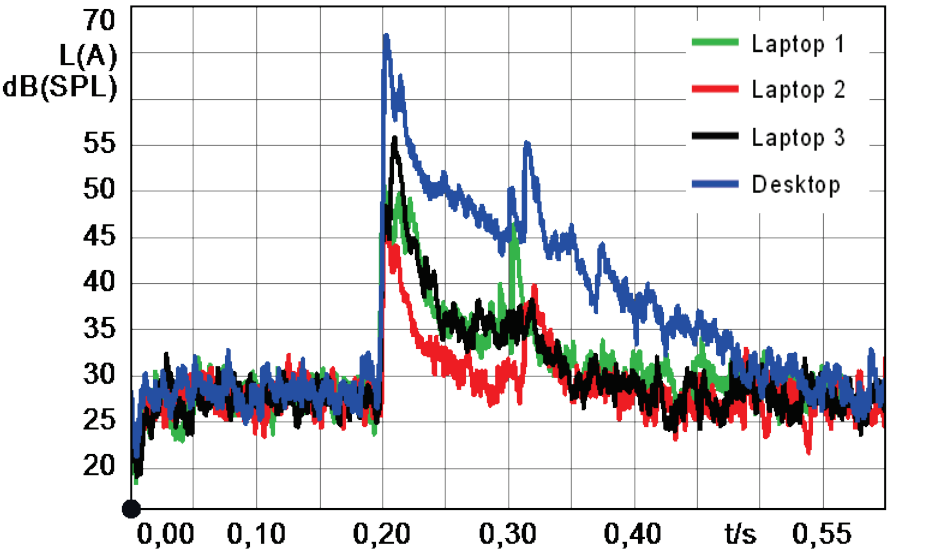
\includegraphics[width=100mm]{TypingSPLKeyboards.png}
\caption{SPL analysis of keyboard noise (time weighting: 2ms). Plot reproduced from \cite{Hauswirth2013}.}\label{fig:TypingSPLKeyboards}
\end{figure}

Figure~\ref{fig:TypingLoudnessKeyboards} shows the loudness of keyboard impulses versus time. Loudness is a representation of a human's perception of sound volume and is represented on a linear scale so that twice the loudness represents a listener perceiving the sound twice as loud. The figure shows that the desktop keyboard is perceived as being over twice as loud as a laptop keyboard. Desktop keyboards are traditionally optimised for typing comfort and tactile feedback while not having to consider the spacial constraints of laptop computers. In addition some keyboards are specifically designed to give the user audible feedback\cite{Hauswirth2013}.

\begin{figure}[!] %TypingLoudnessKeyboards
\centering
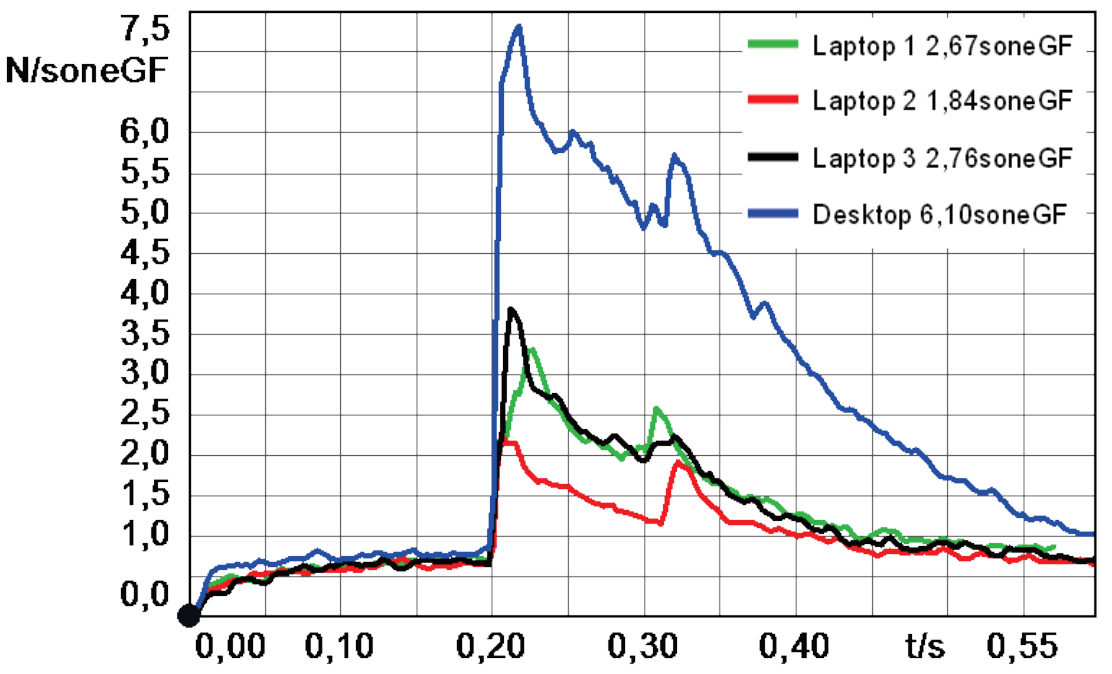
\includegraphics[width=100mm]{TypingLoudnessKeyboards.png}
\caption{Loudness analysis of keyboard noise. Plot reproduced from \cite{Hauswirth2013}.}\label{fig:TypingLoudnessKeyboards}
\end{figure}

In addition to the loudness, Figure~\ref{fig:TypingLoudnessKeyboards} also shows the 5\% percentile value as a single number in the diagram legend. This value indicated the value which the signal exceeds during 5\% of the examined time interval\cite{Hauswirth2013}. This number also reflects the fact that the desktop keyboards in general are perceived much more loudly than laptop keyboards so while laptop keyboards are of interest due to their mechanical connection and physical proximity to the microphone, desktop keyboards is clearly also a potential source of nuisance in telecommunication applications.

\subsection{Spectral investigation of audio signals}
Figure~\ref{fig:spectrogramMarkedTapsBrownFox} shows a spectrogram of a short sequence of speech with typing strokes embedded in it. The figure overlays show the approximate positions of the strokes in the spectrogram. It can be observed that the typing strokes have a fairly flat frequency response compered to the the voiced parts of the audio sequence.

\begin{figure}[!] %spectrogramMarkedTapsBrownFox
\centering
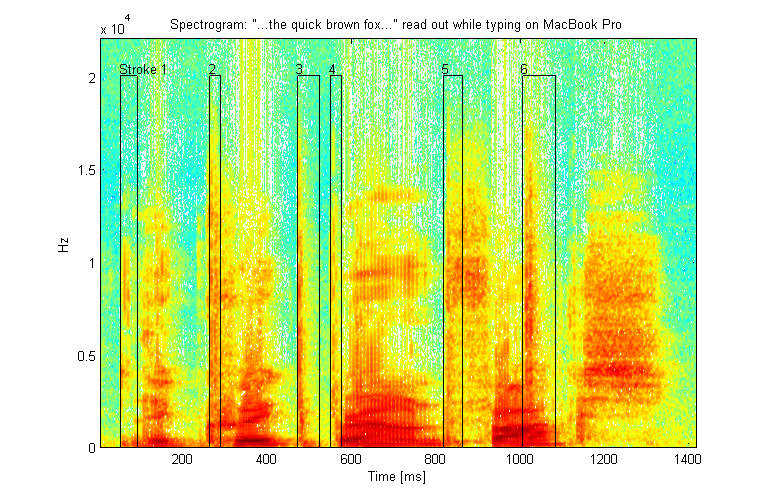
\includegraphics[width=150mm]{spectrogramMarkedTapsBrownFox.png}
\caption{Spectrogram analysis of mixed typing strokes and speech. Overlay shows positions of typing strokes.}\label{fig:spectrogramMarkedTapsBrownFox}
\end{figure}

Figure~\ref{fig:waveletspectrumAno} shows the wavelet spectrum of a sequence of keystrokes with speech interference. The figure overlays show the approximate positions of the strokes in the wavelet spectrum.
\begin{figure}[!] %waveletspectrumAno
\centering
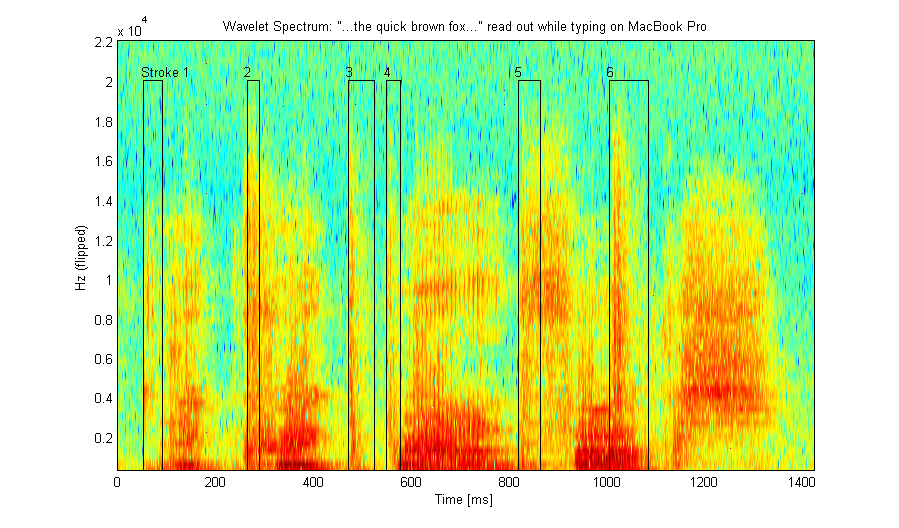
\includegraphics[width=150mm]{waveletspectrumAno.png}
\caption{Top: Waveform of typing sequence. Bottom: Wavelet spectrum of same typing sequence.}\label{fig:waveletspectrumAno}
\end{figure}

\subsection{Keystroke sequence investigation}
A single keystroke, during rapid typing and not at the end of a typing sequence, is generally made up of 3 primary sections.
\begin{enumerate}
  \item A primary \textbf{Stroke} keystroke (15 - 40 ms),
  \item a \textbf{Break} while key is depressed (50 - 500 ms) and
  \item a \textbf{Lift} impulse (15 - 40 ms).
\end{enumerate}
The duration of the break region will typically be determined by the typing speed of the user while the Stroke and the Lift region are primarily constant and will vary more with factors such as stroking force and the vibrational characteristics of the keyboard and the laptop casing.

Figure~\ref{fig:KeyboardStrokeSlow} shows a waveform of a single typing stroke. The waveform clearly shows the two distinct impulses of sudden erratic excitation followed by a slowly decaying low frequency sinusoid.

\begin{figure}[!] %KeyboardStrokeSlow
\centering
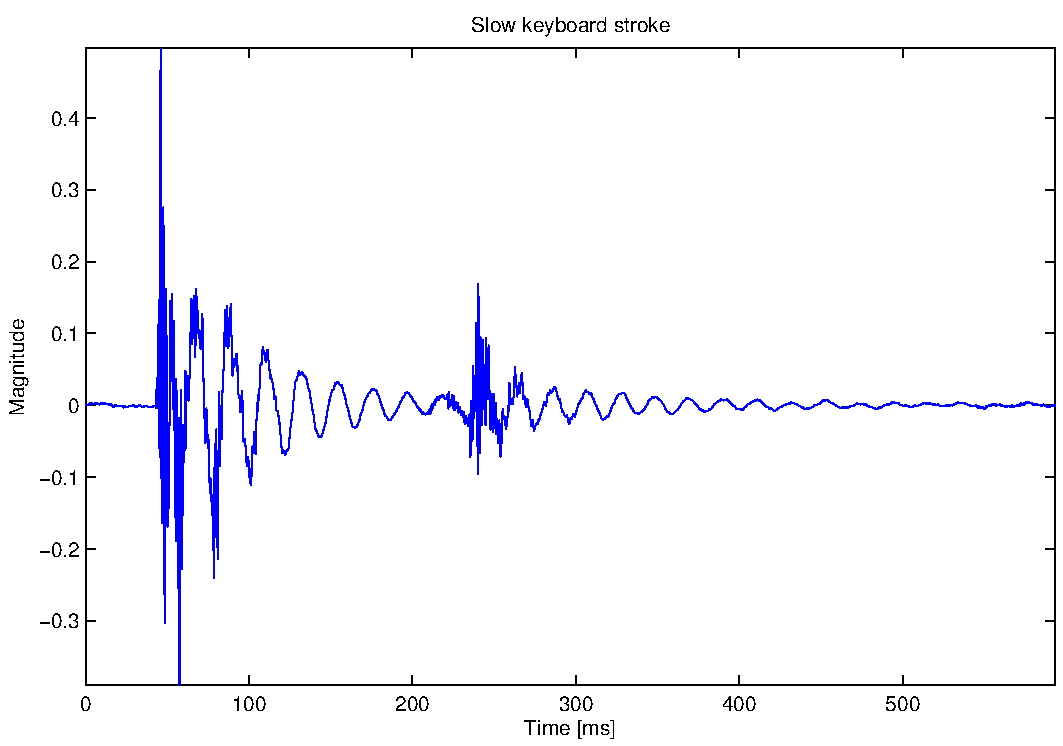
\includegraphics[width=120mm]{KeyboardStrokeSlow.pdf}
\caption{Single slow keyboard stroke.}\label{fig:KeyboardStrokeSlow}
\end{figure}

Figure~\ref{fig:Keyboard2StrokesFast} shows a sequence of two keystrokes in rapid succession. The keystroke regions mentioned above are clearly annotated with their temporal extent also noted.

\begin{figure}[!] %Keyboard2StrokesFast
\centering
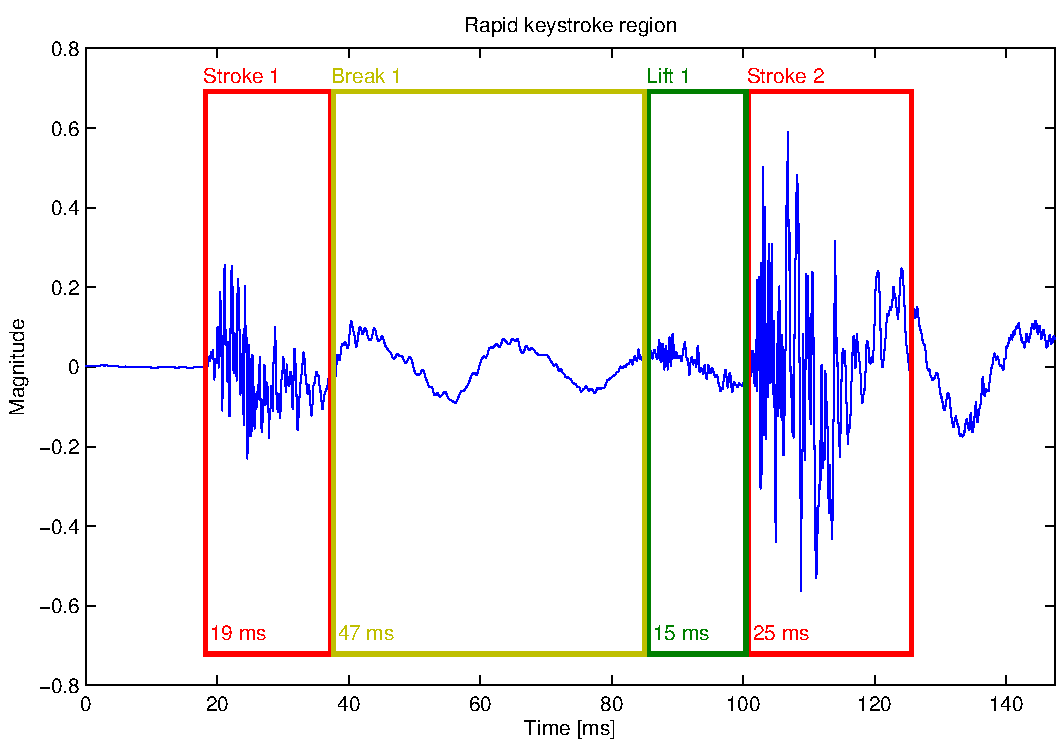
\includegraphics[width=120mm]{Keyboard2StrokesFast.pdf}
\caption{Two annotated keyboard strokes in rapid succession.}\label{fig:Keyboard2StrokesFast}
\end{figure}

Figure~\ref{fig:Keyboard4StrokesFast} shows an example of a short rapid 4 keystroke sequence.

\begin{figure}[!] %Keyboard4StrokesFast
\centering
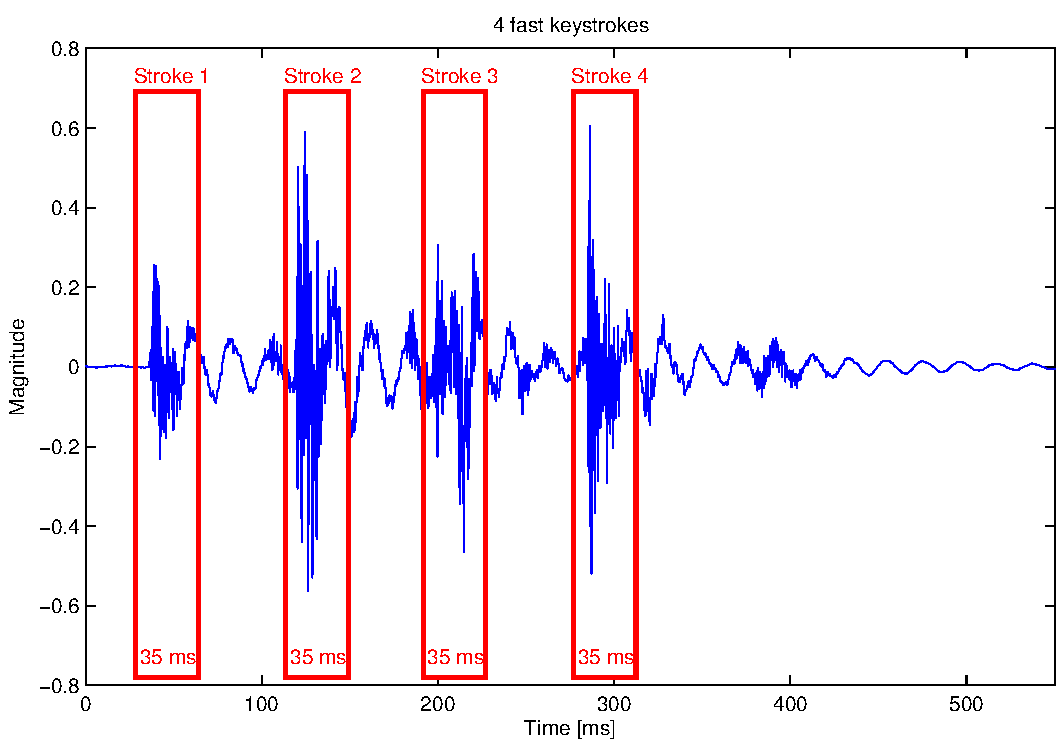
\includegraphics[width=120mm]{Keyboard4StrokesFast.pdf}
\caption{Four annotated keyboard strokes in rapid succession.}\label{fig:Keyboard4StrokesFast}
\end{figure}

\section{Detection algorithms}\label{sec:WPdetection}

The basic detection algorithm is comprised of two stages. First a separation stage aims to separate the transient noise pulses by separating out tonal atoms assumed to be speech components and secondly a detection stage which attempts to detect transient noise events through the wavelet bases. For the detection stage 2 different approaches has been explored.

\subsection{Separation pre processing}
The incoming audio signal can be expressed as the linear combination of a voiced signal and a sparse signal containing the transient noise events:
\begin{equation}\label{eq:modelgeneral}
    x(n) = \sum_i c_i \Phi_i(n) + \sum_{j} w_{j}(n) \Psi_{j}(n),
\end{equation}
where $c_i$ are the coefficients for the voiced parts of the signal and $\Phi$ is the standard short-time Fourier basis. $w_{j}(n)$ are the coefficients of the residual where $j$ is an integer relating to some translation and dilation of some Wavelet basis function $\Psi$. Here we are utilising an overcomplete dictionary of atoms to represent the audio: a dictionary of `tonal' atoms and a dictionary of `transient' atoms that are aimed at capturing voiced speech and transient noise, respectively. Multiple dictionaries have been employed in Bayesian probabilistic methodologies for noise reduction purposes in \cite{Fevotte2006}\cite{Fevotte2008}   (see also references therein for other approaches with multiple dictionaries). We plan to report on such fully Bayesian approaches to our model above in future publications, but here we focus on development of a fast algorithm using the principles of the above model in order to first extract the tonal (voiced) components in order to process the noise components directly in wavelet domain. Other tonal dictionaries such as Gabor functions and other transient dictionaries such as standard discrete or continuous wavelet transforms can of course be substituted in our methods with minor modifications. Wavelets are found to be particularly suited to the types of noise transient we observe here, which are localised in time and can be of highly variable durations and frequency profile.

Figure~\ref{fig:Separation_Residual_Example} shows an example of the residual obtained by simply subtracting outstanding peaks from the spectrum on frames of 20ms with 10ms overlap. The spectral peaks were identified using a threshold of a factor of three of the median filtered spectrum excluding frequencies below 85 Hz and above 10 kHz. The audio data presented in Figure~\ref{fig:Separation_Residual_Example} is a short sentence with two keystrokes embedded in it. The red plot overlay shows the residual where it is clear that the speech magnitude has been greatly reduced while the two clear keystrokes are largely left unchanged. \todo{Numerical justification for the effectiveness of the separation.}

\begin{figure}[htb]
\begin{minipage}[b]{1.0\linewidth}
  \centering
  \centerline{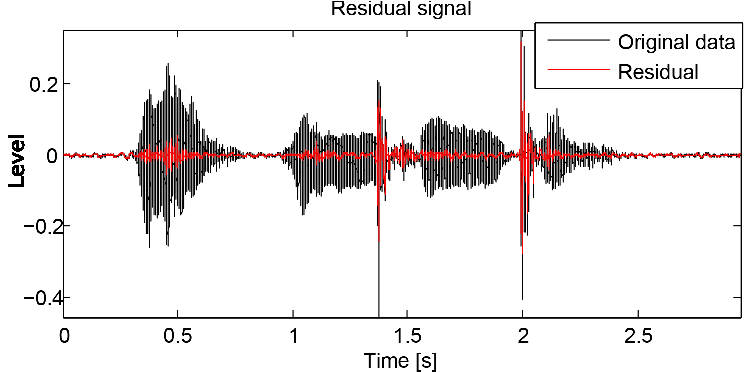
\includegraphics[width=10cm]{Separation_Residual_Example}}
\end{minipage}
\caption{Example of the separation step.}
\label{fig:Separation_Residual_Example}
\end{figure}

The coefficients $w_{j}(n)$ from equation (\ref{eq:modelgeneral}) can be interpreted as wavelet coefficients from a Wavelet Packet Decomposition (WPD) such that $j$ denotes the $j$th terminal node or scale, $j \in \{1, \ldots, J\}$ where $J = L^2$ for an level $L$ decomposition, and $n$ is the time index related to the coefficient set and so $w(n)$ will be used to denote a vector of all coefficients at a given time index $n$. For the case of a wavelet decomposition with decimation steps the time index from the terminal node coefficient sets and equation~\ref{eq:modelgeneral} will be related by a factor of $1/J$.

\todo{Write description of implementation (algorithm)}

\subsection{Noise burst model}
\subsection{AR filtering approach}

% ------------------------------------------------------------------------


%%% Local Variables:
%%% mode: latex
%%% TeX-master: "../thesis"
%%% End:
